\documentclass[a4paper,ngerman]{scrartcl}

\usepackage{amsmath}
\usepackage{amsfonts}
\usepackage{amssymb}
\usepackage[utf8]{inputenc}
\usepackage{graphicx}
\usepackage[ngerman]{babel}
\usepackage{hyperref}
\usepackage{float}
\usepackage{caption}
\usepackage{subcaption}
\usepackage{multirow}  %for tables
\usepackage{icomma} % Handle german comma as decimal point in numbers
\usepackage{units,siunitx} % Write units with correct spacing
\usepackage{upgreek} % provide non-italic greek letters
\usepackage{url}
\usepackage{booktabs}
%\usepackage{subfig}

% Formatting of table & figure captions
\captionsetup{font={sf,footnotesize},labelfont=bf,textfont=sl,skip=6pt}
\setlength{\abovecaptionskip}{6pt}
\setlength{\belowcaptionskip}{0pt}

%locale for units to german
\sisetup{locale = DE}
\sisetup{separate-uncertainty=true}

\title{Landéfaktor\\Versuchsauswertung}
\date{\today}
\author{Michel Rausch, Michael Eliachevitch}

\begin{document}

\maketitle
\tableofcontents
\newpage

\section{Zeitkalibrierung}

Ein Funktionsgenerator wurde an den Starteingang des TAC geschlossen, sowie über Verzögerungsglieder an des Stoppeingang. Diese wurden zugeschaltet, um die Zeitverzögerung in bekannten Schritten von $\SI{1}{\nano \second}$ zu erhöhen. Die zugehörigen Peaks waren scharf gegenüber dem Abstand, sodass die Messungen in einer einzelnen Grafik, Abb. \ref{fig:zeitkalibrierung_hist}, auswerten ließen. Die Nummer des Kanals steigt mit der zugehörigen Verzögerung. 

\begin{figure}[tb!]
\centering
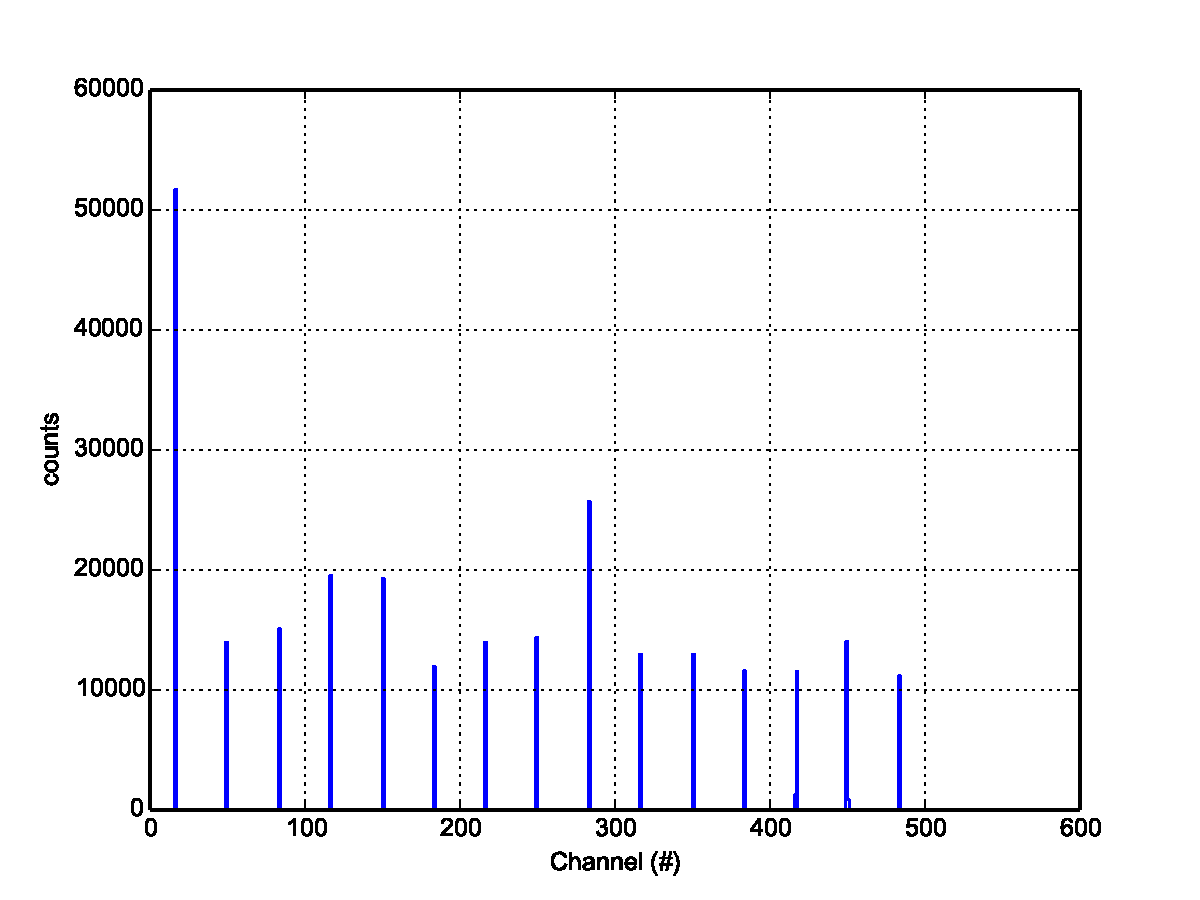
\includegraphics[width=0.7\textwidth]{abbildungen/zeitkalibrierung_hist.pdf}
\caption[Daten zur Zeitkalibrierung]{\textbf{Daten zur Zeitkalibrierung.} Die gezeigten Peaks gehören zu unterschiedlichen Verzögerungen. Die zugehörigen Peaks waren scharf gegenüber dem Abstand, sodass die Messungen in einer einzelnen Grafik auswerten ließen. Die Verzögerung wird von dem Peak am weitesten links nach rechts schrittweise um $\SI{1}{\nano \second}$ größer.}
\label{fig:zeitkalibrierung_hist}
\end{figure}


Die Zeit wurde den Kanälen zugewiesen. Mit Python wurde eine lineare Regression durchgeführt. Mit der resultierenden Geradengleichung wurden die Kanäle einer Zeit zugewiesen. Die Regression ist in Abbildung \ref{fig:zeitkalibrierung} gezeigt, das Ergebnis lautet

\begin{equation}
\label{eqn:Zeitkalibrierung}
\frac{\mathrm{Zeit}}{\mathrm{Kanal}} = \SI{2.99783924  \pm 0.00000004 }{\pico \second} ~.
\end{equation}


\begin{figure}[tb!]
\centering
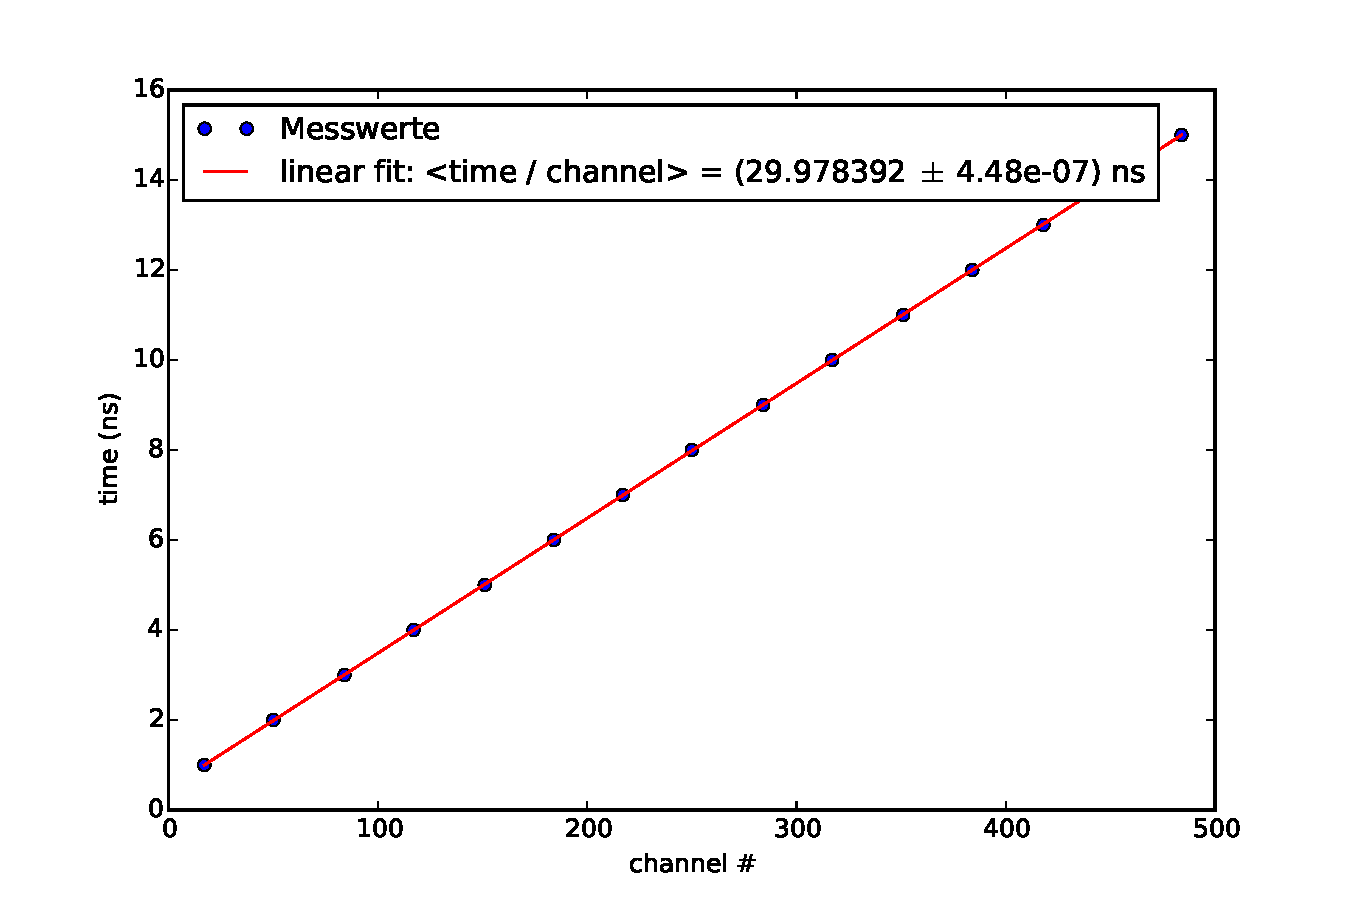
\includegraphics[width=0.7\textwidth]{abbildungen/zeitkalibrierung.pdf}
\caption[Zeitkalibrierung]{\textbf{Zeitkalibrierung.} Mittels eines Pythonscripts wurde ein linearer Fit durchgeführt. Die Kanalnummer des VKAs wurde auf der x-Achse aufgetragen, die dazugehörige Verzögerung auf der y-Achse. Mit der Geradengleichung wurden Kanäle einer Zeit zugeordnet.}
\label{fig:zeitkalibrierung}
\end{figure}





\section{Magnetfeld}

Das Magnetfeld wurde mit einer Hallsonde bestimmt. Aus den Daten der Kalibrierung, die übernommen wurde, konnte die gemessene Spannung am Vorwiderstand $U_{\mathrm{VW}}$ in die Magnetfeldstärke umgerechnet werden. Zur Umrechnung wurde 

\begin{equation}
\label{eqn:B-gauss}
B \mathrm{/G} = -1,68946 + 0,30472 \cdot U_{\mathrm{VW}} \mathrm{/mV}
\end{equation}

verwendet. In der Spule ist das Magnetfeld inhomogen. Der Fehler für die Inhomogenität wurde aus der übernommenen Messreihe in Tabelle \ref{tab:fieldinhomogenities} ermittelt. Es sind die Spannungen an der Hallsonde aufgelistet. Diese stehem in einem linearen Verhältnis zu der Magnetfeldstärke, daher können die relativen Fehler übernommen werden. Der relative Fehler für jeweils vier Werte, also für jeden Punkt entlang der Spule wurde bestimmt. Über diese wurde gemittelt, um den mittleren relativen Fehler zu bestimmen. Dieser war

\begin{equation}
\label{eqn:inhomogen_fehler}
\sigma_{\mathrm{B}} = 0,02 = 2 \% ~.
\end{equation}

Die Spannung am Vorwiderstand betrug

\begin{equation}
U_{\mathrm{VW}} = \SI{123,6}{\milli \volt} ~.
\end{equation}

Hieraus ergab Formel \eqref{eqn:B-gauss}, mit dem Fehler für die Inhomogenität aus Gleichung \eqref{eqn:inhomogen_fehler},
\begin{equation}
B = \SI[separate-uncertainty=true]{36.0 \pm 0.7 }{G} ~.
\end{equation}

\begin{table}[tb!]
\centering
\caption[Inhomogenität des Magnetfelds der Spule]{\textbf{Inhomogenität des Magnetfelds der Spule} Um den relativen Fehler zum Magnetfeld zu finden wurde auf vorliegende Messungen einer Hallsonde zurückgegriffen. Über verschiedene Punkte an der Länge $l$ der Spule wurde die Spannung an der Hallsonde gemessen. Für jeden dieser Punkte wurden vier Messwerte für verschiedene Positionen innerhalb des Spulenquerschnitts aufgenommen. Die mit "'*"' markierten Werte für $l = \SI{0.00}{m}$ und $l = \SI{1.00}{m}$ wischen stark von den anderen Werten ab, wurden daher nicht in die Berechnung des Fehlers aufgenommen.}
\begin{tabular}{ccccc}
\toprule 
$l$/m	&	$U_{\mathrm{Hall}} (0 \mathrm{m})$/mV	&	$U_{\mathrm{Hall}} (0,28 \mathrm{m})$/mV	&	$U_{\mathrm{Hall}}(- 0,28 \mathrm{m})$/mV	&	$U_{\mathrm{Hall}} (0 \mathrm{m})$/mV	\\
\midrule
0,00* & 149,6* & 123,6* & 123,6* & 139,7* \\
0,05 & 213,9 & 231,2 & 227,5 & 218,8 \\
0,10 & 243,6 & 257,1 & 257,2 & 243,6 \\
0,15 & 247,3 & 267,0 & 267,0 & 248,5 \\
0,20 & 253,4 & 271,0 & 272,0 & 249,7 \\
0,25 & 272,0 & 279,4 & 279,4 & 262,1 \\
0,30 & 288,1 & 284,3 & 285,6 & 291,8 \\
0,35 & 283,1 & 283,1 & 284,3 & 284,3 \\
0,40 & 270,7 & 279,4 & 281,9 & 270,7 \\
0,45 & 269,5 & 279,4 & 280,6 & 269,5 \\
0,50 & 279,4 & 280,6 & 283,1 & 278,2 \\
0,55 & 289,3 & 283,1 & 285,6 & 290,5 \\
0,60 & 289,3 & 284,3 & 285,6 & 289,3 \\
0,65 & 264,6 & 278,2 & 278,2 & 260,9 \\
0,70 & 273,2 & 279,4 & 280,6 & 273,2 \\
0,75 & 270,7 & 280,6 & 280,6 & 274,5 \\
0,80 & 259,6 & 274,5 & 274,5 & 257,2 \\
0,85 & 255,9 & 272,0 & 270,7 & 257,2 \\
0,90 & 243,6 & 262,1 & 260,9 & 244,8 \\
0,95 & 217,6 & 238,6 & 237,4 & 222,5 \\
1,00* & 157,0* & 160,7* & 155,8* & 163,2* \\
\bottomrule
\end{tabular}
\label{tab:fieldinhomogenities}
\end{table}








\section{Bestimmung der Lebensdauer des Myons}









\section{Bedeutung des Landéfaktors}

Der Landéfaktor $g$ gibt für ein Teilchen das Verhältnis des gemessenen magnetischen Moments $ u_{\mathrm{gemessen}}$ zu dem klassisch erwartetem magnetischem Moment $u_{\mathrm{klassisch}}$ an. Demnach gilt

\begin{equation}
g = \frac{ u_{\mathrm{gemessen}} }{u_{\mathrm{klassisch}} } ~.
\end{equation}

Jeder Drehimpuls besitzt in einem Magnetfeld ein magnetisches Moment. Für unterschiedliche Drehimpulse können die Landéfaktoren voneinander abweichen. So ist $g$ für den Bahndrehimpuls eines geladenes Teilchens genau eins, für dessen Spin jedoch $2 + \text{Korrekturen höherer Ordnung}$. Auch negative Werte sind möglich.

\begin{equation}
g = \frac{\hbar \omega}{\mu_B B} ~.
\end{equation}

\section{Bestimmung des Landéfaktors des Myons}




\section{Diskussion der Ergebnisse}




\section{Quellen}
\begin{enumerate}
\item Vorbereitungsmappe 
\end{enumerate}



\end{document}
